\section{Performance Evaluation}
\label{sec:evaluation}

We evaluate the protocols along four latency-oriented axes mapping to the questions of Section~\ref{sec:intro}: session-setup latency, command completion (W1), large-output delivery (W2), and interactive keystroke latency (W3), and on output completeness. Figure~\ref{fig:session-setup}, Figure~\ref{fig:workload-latency-steady}, and Table~\ref{tab:recv-pct} report the results. Each per-workload latency is a macro-average over the commands in that workload.

% \begin{figure*}[t]
%     \centering
%     \subfloat[W1: Small-output]{%
%         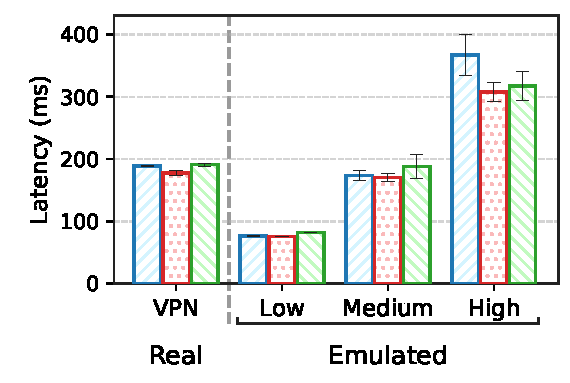
\includegraphics[width=0.48\textwidth]{figs/latency_w1_by_scenario.pdf}%
%         \label{fig:latency-w1}
%     }\hfill
%     \subfloat[W2: Large-output]{%
%         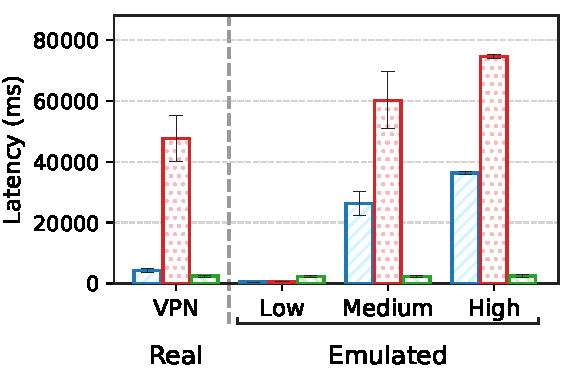
\includegraphics[width=0.48\textwidth]{figs/latency_w2_by_scenario.pdf}%
%         \label{fig:latency-w2}
%     }\\[1ex]
%     \subfloat[W3-1p: Single-pane]{%
%         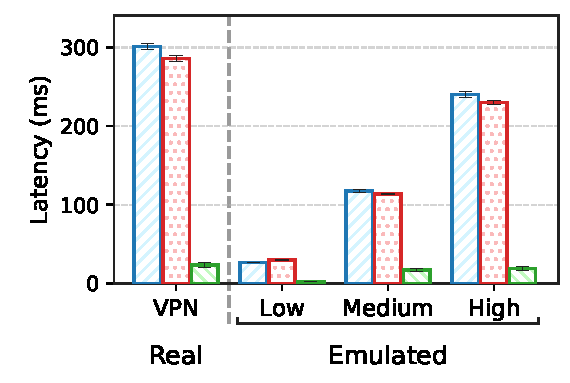
\includegraphics[width=0.48\textwidth]{figs/latency_w3_1p_by_scenario.pdf}%
%         \label{fig:latency-w3-1p}
%     }\hfill
%     \subfloat[W3-5p: Five-pane]{%
%         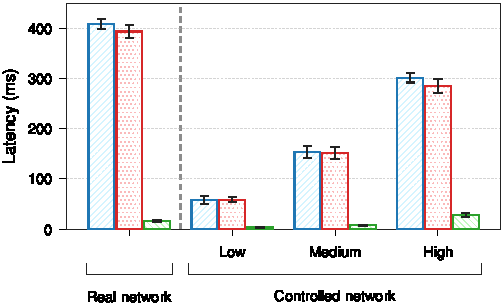
\includegraphics[width=0.48\textwidth]{figs/latency_w3_5p_by_scenario.pdf}%
%         \label{fig:latency-w3-5p}
%     }
%     \caption{Mean latency and 95\% confidence interval (CI 95\%) for the steady-state workloads (excluding warmup samples) across protocols and network scenarios.}
%     \label{fig:workload-latency-steady}
% \end{figure*}
\captionsetup{font=normalsize}
\captionsetup[subfloat]{font=normalsize}
\begin{figure*}[t]
    \centering
    
\includegraphics[width=0.36\textwidth]{figs/latency_workload_legend.pdf}\\[-0.5ex]
    \subfloat[W1: Small-output]{%
        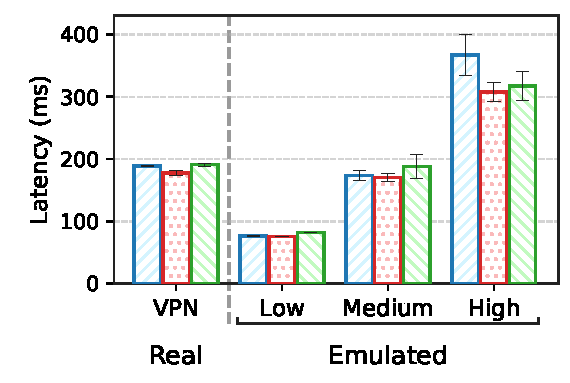
\includegraphics[width=0.47\textwidth]{figs/latency_w1_by_scenario.pdf}%
        \label{fig:latency-w1}
    }\hfill
    \subfloat[W2: Large-output]{%
        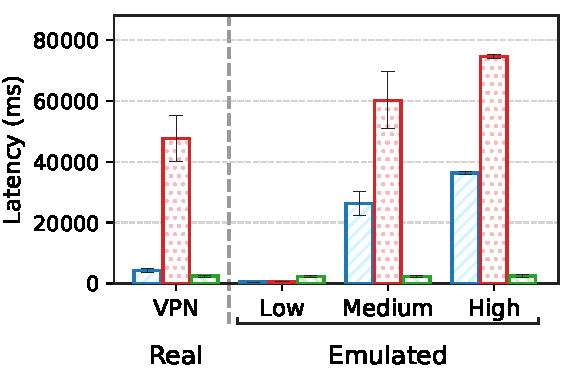
\includegraphics[width=0.47\textwidth]{figs/latency_w2_by_scenario.pdf}%
        \label{fig:latency-w2}
    }\\[-0.5ex]
    \subfloat[W3-1p: Single-pane]{%
        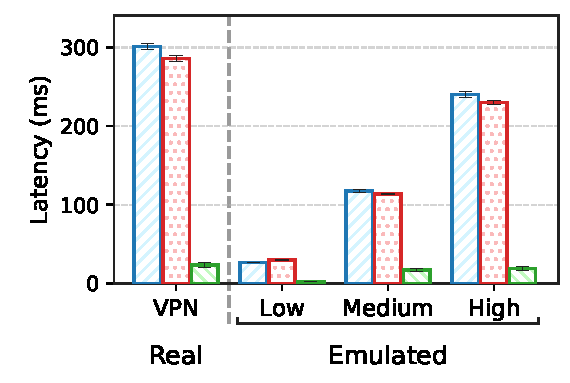
\includegraphics[width=0.47\textwidth]{figs/latency_w3_1p_by_scenario.pdf}%
        \label{fig:latency-w3-1p}
    }\hfill
    \subfloat[W3-5p: Five-pane]{%
        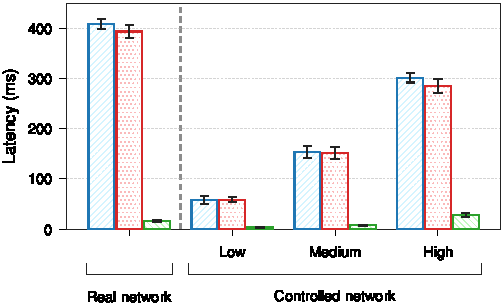
\includegraphics[width=0.47\textwidth]{figs/latency_w3_5p_by_scenario.pdf}%
        \label{fig:latency-w3-5p}
    }
    \captionsetup{font=normalsize}
    \caption{Mean latency and 95\% confidence interval (CI 95\%) for the steady-state workloads (excluding warmup samples) across protocols and network scenarios.}
    \label{fig:workload-latency-steady}
    \captionsetup[subfloat]{font=normalsize}
\end{figure*}
\captionsetup{font=normalsize}
\captionsetup[subfloat]{font=normalsize}


\begin{figure}[h]
    \centering
    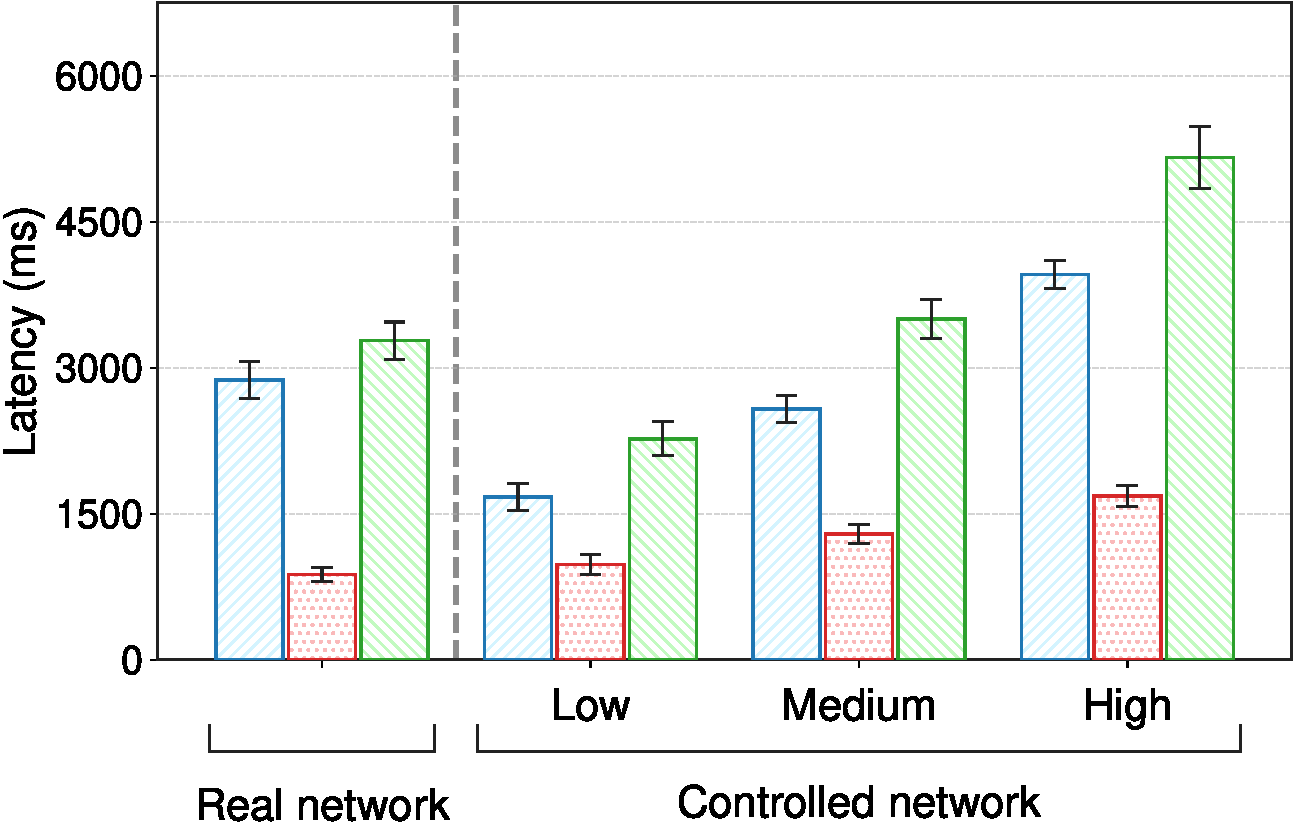
\includegraphics[width=\columnwidth]{figs/session_setup_bar.pdf}
    \caption{Mean session setup latency across four network scenarios.}
    \label{fig:session-setup}
\end{figure}

\subsection{Session Setup Latency}
\label{subsec:session-setup}

We measure session setup as the time from client process spawn to the first interactive shell prompt in Section~\ref{subsec:measurement-metrics}, pooled across all sessions of each (protocol, scenario) configuration (N = 400).

Figure~\ref{fig:session-setup} shows that SSH3 achieves the lowest setup latency in every scenario. In the VPN scenario it establishes a session in 219\,ms, versus 765\,ms for SSHv2 and 908\,ms for Mosh. The same ordering holds under impairment, reaching 1042\,ms vs.\ 3565\,ms and 3856\,ms in the High scenario. This follows from protocol design: SSH3 uses QUIC's 1-RTT handshake, which folds transport setup and key exchange into one round trip \cite{michel2023,Iyengar2021}, whereas SSHv2 needs a TCP handshake plus SSH key exchange and authentication \cite{Ylonen2006RFC4253}. Mosh incurs the highest setup cost because it first completes a full SSHv2 session to bootstrap its UDP-based SSP channel \cite{Winstein2012}.

\subsection{Workload Latency Results}

\paragraph{W1}
We first evaluate completion latency for three sub-kilobyte static fixture commands. SSH3 achieves the lowest mean latency in all four scenarios, although the gap is modest in the Low and Medium cases. In the VPN scenario, SSH3 completes a command loop in 177.9\,ms, compared with 188.8\,ms for SSHv2 and 190.9\,ms for Mosh, corresponding to reductions of 5.8\% and 6.8\%. Under Low impairment, SSH3 and SSHv2 are nearly tied (75.5\,ms vs.\ 76.1\,ms), while Mosh is slower at 82.2\,ms. The benefit becomes clearer as impairment increases: under the High scenario, SSH3 reaches 307.5\,ms, ahead of Mosh at 317.3\,ms and SSHv2 at 367.0\,ms. Since W1 responses are small and content-complete for the successful samples, the measured latency primarily captures request-response delay inside an already established session rather than bulk transfer throughput. The results therefore indicate that SSH3 provides the best steady-state command-loop latency for small outputs in this environment, while Mosh's screen-state synchronization offers little advantage for these byte-complete sub-kilobyte responses.

\paragraph{W2}
Next, we compare large-output delivery using static fixtures that emulate byte-heavy command output. In contrast to W1, the ranking changes once the client must receive hundreds of KiB to MiB of terminal output. Mosh often reports the lowest apparent completion latency (e.g., 2402.4\,ms over VPN and 2467.9\,ms under High impairment), but this latency must be interpreted together with output completeness: Mosh receives only a small fraction of the expected bytes for these fixtures, because SSP synchronizes terminal screen state rather than every byte in the stream \cite{Winstein2012}. Among byte-complete transports, SSHv2 is faster than SSH3 in the comparable W2 cases: over VPN SSHv2 completes in 4213.5\,ms versus 47732.6\,ms for SSH3, and under Medium impairment in 26353.2\,ms versus 60207.2\,ms. Under High impairment, SSH3 successfully completes the small and medium fixtures but times out on the large fixture in this result set; therefore its 54320.0\,ms aggregate excludes the hardest case and should not be directly compared with SSHv2's 77422.6\,ms aggregate over all three fixtures. On the common small and medium High fixtures, SSHv2 remains faster. This is consistent with prior QUIC measurements showing that QUIC's advantage over TCP is workload-, path-, and implementation-dependent rather than universal \cite{Kakhki2017,Langley2017}. Moreover, QUIC removes head-of-line blocking across independent streams, but SSH3 maps each channel onto a QUIC stream whose messages still require in-order delivery; within such a single ordered stream, lost stream data is retransmitted before the byte stream can be completed \cite{michel2023,Iyengar2021}. These results show that, for single-stream bulk terminal output in our implementation and network setup, SSHv2 provides the most reliable byte-complete W2 delivery, whereas Mosh's low latency reflects responsiveness after partial screen-state synchronization rather than complete output arrival.

\paragraph{W3}
Finally, we consider the keystroke-to-echo latency in both single-pane and five-pane tmux layouts. It is shown that Mosh achieves the best performance in every scenario and layout, especially under degraded network conditions. For instance, under the High scenario, Mosh maintains a latency of 25.3-31.3\,ms, which is significantly lower than that of SSHv2 and SSH3 (both exceeding 220\,ms). This gap is driven by Mosh's local echo and predictive rendering, which hide part of the network delay. Furthermore, when comparing SSH3 and SSHv2, SSH3 improves the latency over VPN (achieving 2.1\,ms vs.\ 20.2\,ms in the single-pane layout, and 9.4\,ms vs.\ 23.9\,ms in the five-pane layout). However, under the Low scenario, SSH3 becomes slightly worse than its SSHv2 counterpart for both layouts (e.g., 29.3\,ms vs.\ 26.1\,ms for single-pane). This indicates that QUIC does not substantially reduce steady-state keystroke latency once network delay dominates the per-character path. Besides, moving from one to five panes significantly slows down SSHv2 and SSH3 under impairment due to increased network-crossing screen updates, whereas Mosh is largely unaffected. This is consistent with Mosh's update coalescing and local prediction, making it the most responsive protocol for interactive workloads.

\subsection{Output Completeness}
\label{subsec:output-completeness}

\begin{table}[t]
\centering
\caption{Output completeness, measured as the percentage of expected bytes received by the client.}
\label{tab:recv-pct}
\renewcommand{\arraystretch}{1.15}
\begin{tabular}{llrrrr}
\hline
\textbf{Workload} & \textbf{Protocol} & \textbf{VPN} & \textbf{Low} & \textbf{Medium} & \textbf{High} \\
\hline
\multirow{3}{*}{\textbf{W1 (\%)}} 
 & \textbf{SSHv2} & 100.00 & 100.00 & 100.00 & 100.00 \\
 & \textbf{SSH3}  & 100.00 & 100.00 & 100.00 & 100.00 \\
 & \textbf{Mosh}  & 100.00 & 100.00 & 100.00 & 100.00 \\
\hline
\multirow{3}{*}{\textbf{W2 (\%)}} 
 & \textbf{SSHv2} & 100.00 & 100.00 & 100.00 & 100.00 \\
 & \textbf{SSH3}  & 100.00 & 100.00 & 100.00 & 100.00 \\
 & \textbf{Mosh}  & 1.43 & 4.19 & 1.75 & 1.24 \\
\hline
\end{tabular}
\end{table}

Output completeness measures whether the client receives the expected output. Table~\ref{tab:recv-pct} reports the mean percentage of received bytes, comparing captured output against static fixture references. For W1, all three protocols receive 100\% of the expected bytes across all scenarios, showing that sub-kilobyte command outputs are small enough for Mosh's screen synchronization to preserve the full visible response in successful samples. The W2 result is sharply different. SSHv2 and SSH3 receive 100\% of the expected bytes in every scenario, and the follow-up SHA-256 validation confirms content matches for their successful samples. Mosh receives only a small fraction of the large-output fixtures: 1.43\% over VPN, 4.19\% under Low impairment, 1.75\% under Medium, and 1.24\% under High. This matches SSP's design, which synchronizes the visible screen state rather than every byte, so when updates arrive faster than the frame interval, intermediate output states are skipped and only the latest screen is sent.

This is acceptable for human use, where the final visible screen matters more than byte-level completeness, but problematic for agents, which parse output to read file listings, process lists, errors, or system state: skipped output can make the agent act on incomplete data. Hence Mosh can be responsive for interactive viewing, but SSHv2 and SSH3 are the reliable choices when byte-complete and content-correct large output is required.

